\documentclass[12pt,a4paper,titlepage,twoside]{book}
\usepackage{chngcntr}
\usepackage[bottom]{footmisc}
\usepackage[applemac]{inputenc}
\usepackage[italian]{babel}
\usepackage{guit}
\usepackage[autostyle, italian=guillemets]{csquotes}
\usepackage[T1]{fontenc}
\usepackage{graphicx}
\usepackage{setspace}
\usepackage{frontespizio}
\usepackage{imakeidx}
\usepackage{midpage}
\makeindex[]
\begin{document}

	\begin{flushleft}
		\large
		\textsc{Giulia Franco} \\
		\textsc{matricola SM3500370}\\
		\textsc{Year 2018/2019}
		\\
		\textsc{Exercise 1,Parallel Computing course.}
	\end{flushleft}
\newpage
\begin{figure}
	\section*{Computing pi using OpenMPI}
	The aim of the exercise is to compute $\pi$ using midpoints rule in a OpenMPI approach. The computation is done using the same algorithm as in OpenMP, collecting the processes results using "$MPI\_Reduce$" function into the last process available.\\
	The final result is then sent from the last process to the first one using "$MPI\_Send$" and "$MPI\_Recv$", and finally printed.\\
	Time of execution is calculated for different number of processes in order to  underlining the gain in performance. The result is represented in the following graph.
	\begin{center}
		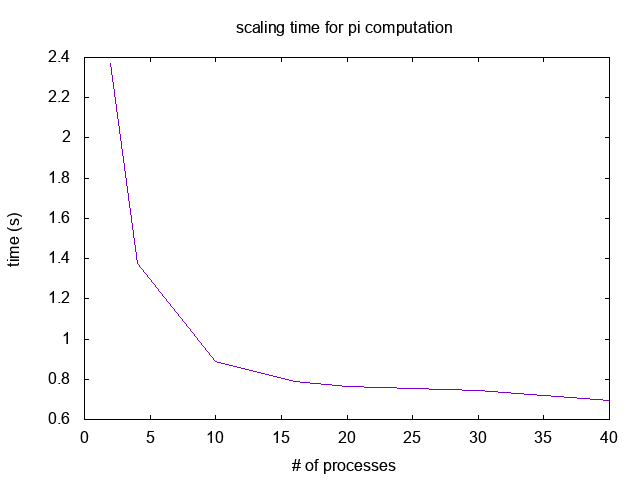
\includegraphics[height=80mm, ]{mpi_p_timing}
	\end{center}
	\section*{Compiling and Executing exercises} 

The first step on Ulysses is to reserve two nodes for the execution:

\underline{qsub -l nodes=2:ppn=20 -I -l walltime=1:00:00}.\vspace{0.5cm}

Then compiling using:\\
module load openmpi\\
mpicc $mpi\_p.c$ -o $mpi\_p$\vspace{0.5cm}
\\Finally executing using the script in the current folder:\\
./cases.sh\vspace{0.5cm}
\end{figure}
\end{document}